\documentclass[11pt, oneside]{article} 
\usepackage{geometry}
\geometry{letterpaper} 
\usepackage{graphicx}
	
\usepackage{amssymb}
\usepackage{amsmath}
\usepackage{parskip}
\usepackage{color}
\usepackage{hyperref}

\graphicspath{{/Users/telliott_admin/Dropbox/Tex/png/}}
% \begin{center} 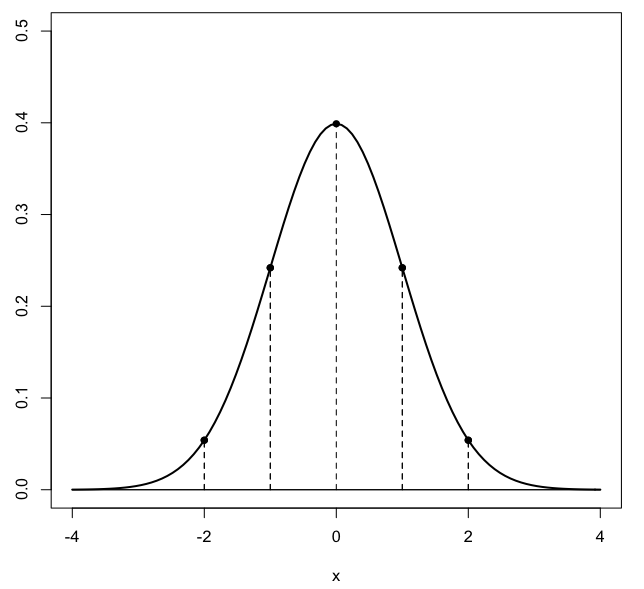
\includegraphics [scale=0.4] {gauss3.png} \end{center}

\title{Introduction to Green's Theorem}
\date{}

\begin{document}
\maketitle
\Large

\label{sec:green}

\subsection*{flux and curl}

We now undertake an exploration of the fundamental theorems of vector calculus.

First, though, a word about flux and curl.  Flux seems pretty clear:  it is the flow out of a region, across a line in $\mathbb{R}^2$ or across a surface in $\mathbb{R}^3$.

Curl, on the other hand, measures the rotation of a vector field (its absolute value is twice the angular momentum).  

As an example, if a two dimensional field $\mathbf{F}$ has components $\ \langle M,N \rangle \ $, then
\[ \text{curl} \ \mathbf{F} = N_x - M_y \]

Note:  we write $M,N$ for the components of a field in $\mathbb{R}^2$ and $P,Q,R$ for the components of a field in $\mathbb{R}^3$

As we'll see, the result of $\text{curl} \ \mathbf{F}$ is a vector, in this case it points out of the plane.  When we calculate with it in 2D we are implicitly forming the dot product with $\hat{\mathbf{k}}$ and then ignoring the third dimension.

\subsection*{right-hand rule}

Our convention is that we go on a curve around a region with that region $R$ on our left, and then the curl points up.  This is a result of what is called the "right hand rule."

If the value of $\text{curl} \ \mathbf{F}$ is zero, then the work done going around a closed curve is also zero, alternatively if the curl is non-zero, work is done.  Think of swimming in a whirlpool.

Against the flow it is hard going, whereas with the flow, it's easy.

In our theorems, the curl will be associated with the line integral for work.  The work done in moving along a curve $C$ is

\[ W = \int_C \mathbf{F} \cdot d\mathbf{r}  \]

\subsection*{Del:  $\nabla$}

In three dimensions, we introduce the "del" operator
\[ \nabla = \ \ \langle \frac{\partial}{\partial x},\frac{\partial}{\partial y},\frac{\partial}{\partial z}  \rangle \  \]

$\nabla$ is used in several ways.  The first is to indicate the gradient or "grad" of a scalar function $f(x,y,z)$.  The result is a vector field:
\[ \mathbf{F} = \nabla f = \ \langle f_x, f_y, f_z \rangle \]

$\nabla$ is also used to indicate the \emph{divergence} of a vector field $\mathbf{F}$.  

\[ \nabla \cdot \mathbf{F} \]
\[ = \ \langle \frac{\partial}{\partial x},\frac{\partial}{\partial y},\frac{\partial}{\partial z}  \rangle \ \cdot \ \langle P, Q, R \rangle \]
\[ =  \ \langle P_x, Q_y, R_z \rangle \]

The third use is for the curl of $\mathbf{F}$, which is written as
\[ \nabla \times \mathbf{F} \]

and defined 

\[ \nabla \times \mathbf{F} =  \ \ \langle R_y-Q_z,P_z-R_x,Q_x-P_y \rangle \  \]
which is basically impossible to remember except by using this convenient device
\[
\begin{vmatrix} 
  \hat{i}  &  \hat{j} & \hat{k} \\ 
  \frac{\partial}{\partial x}  &  \frac{\partial}{\partial y} & \frac{\partial}{\partial z} \\ 
  P  & Q & R \\ 
\end{vmatrix} \ \
\]
We think of forming the "determinant" of this "matrix."

In two dimensions $R=0$ and also $P_z$ and $Q_z$ are both zero so
\[ \nabla \times \mathbf{F} = \langle 0,0,Q_x-P_y \rangle \  \]
or substituting the symbols usually used for the field components in $\mathbb{R}^2$, we have

\[ \nabla \times \mathbf{F} = N_x - M_y \]

This is the equation we saw above.

A basic fact in vector calculus is that \textbf{if the field is the gradient of a potential function, the curl is zero}.  

Let the function be $f$ and the field $\mathbf{F} = \nabla f$, then $M=f_x$ and $N=f_y$.  Then the curl is $f_{yx}- f_{xy}$, but for any such function
\[ f_{xy} = f_{yx} \]

Equivalent formulations of this are that 

$\circ \ \ \ $ the work integral is independent of the path

$\circ \ \ \ $ the integral around any closed path is zero.

\subsection*{Calculations}
Let's look again at
\[ W = \int_C \mathbf{F} \cdot d\mathbf{r}  \]
This can be written as
\[ = \int_C M \ dx + N \ dy  \]

(It can also be written as
\[ = \int_C \mathbf{F} \cdot ds \mathbf{\hat{T}}   \]
where $\mathbf{\hat{T}}$ is the tangential vector in the direction of motion, in the same direction as the velocity $\mathbf{v}$).

One way to see $\int_C M \ dx + N \ dy$ is to say
\[ d\mathbf{r} = \frac{d}{dt} \mathbf{r} \ dt = \ \langle \frac{dx}{dt},\frac{dy}{dt} \rangle \  \ dt = \ \langle dx,dy \rangle \]
so when we do the dot product with $\mathbf{F}$, we get what is written above.

There is another important integral to be explained below (the one for flux):
\[ \int_C \mathbf{F} \cdot \hat{\mathbf{n}} \  ds = \int_C -N \ dx + M \ dy  \]
Notice the similar form with the first one.  It is also helpful to remember that the unit tangential vector $\mathbf{\hat{T}}$ and the unit normal vector $\mathbf{\hat{n}}$  are orthogonal.

Although these equations look something like a double integral, they are \emph{not}.

We will have a parametrization of the curve in terms of $t$ (or $x$ or $\theta$), and a single integral like $\int_C f(t) \ dt $.

\subsection*{Green---work}
We start with two theorems in the plane (typically the $xy$-plane).  These are called Green's Theorem for work, and Green's Theorem for flux.  

Green's Theorem for work states that for a closed path

\[ \oint \mathbf{F} \cdot d\mathbf{r}  = \iint_R \ \nabla \times \mathbf{F} \ dA \]

One sticky point I had here is that the curl produces a vector, yet the formula is usually given as above.  That's because this is a special case of Stokes theorem where the term on the right is really 
\[ (\nabla \times \mathbf{F}) \cdot \hat{\mathbf{k}} \ dA \]
which (since $\nabla \times \mathbf{F} $ is parallel to $\hat{\mathbf{k}}$) gives what we have above.

Alternatively (and best to remember for computation):

\[ \int_C M \ dx + N \ dy = \iint_R (N_x - M_y) \ dx \ dy \]

The work done along a closed path around $R$ is equal to the double integral over $R$ of the curl of $\mathbf{F}$.  

Remember the whirlpool.

\subsection*{Green---flux}
The theorem for work can be reformulated to give a new result, about flux or flow across the curve.

Flux is flow across a curve, or in $\mathbb{R}^3$, through a surface.

Green's Theorem for flux in the plane states that for a closed path $C$ over a region $R$

\[ \int_C \mathbf{F} \cdot \hat{\mathbf{n}} \  ds = \iint_R \ \nabla \cdot \mathbf{F} \ dA \]
where the expression on the left is a line integral, and the quantity on the right is the integral of the divergence of $\mathbf{F}$, symbolized with the "del" operator.

Alternatively
\[ \int_C M \ dy - N \ dx =  \iint_R \ (M_x + N_y) \ dx \ dy \]

\[ \nabla \cdot \mathbf{F} \]
if $\mathbf{F} = \ \ \langle M,N \rangle \ $
\[ \nabla \cdot \mathbf{F} = M_x + N_y \]

The divergence of a vector field is a scalar quantity.  It measures the net production (or disappearance) of the "substance" that flows in a vector field.  If there are no sources or sinks in a region, the divergence of $\mathbf{F}$ will be zero.

Restating the theorem:

\[ \oint \mathbf{F} \cdot \hat{\mathbf{n}} \ dS  = \iint_R \ \nabla \cdot \mathbf{F} \ dA \]

Breaking this down, on the left hand side=, $\hat{\mathbf{n}}$ is the unit vector \emph{orthogonal} to $\hat{\mathbf{T}}$.  Since $\hat{\mathbf{n}}$ and $\mathbf{n}$ are orthogonal to $\hat{\mathbf{T}}$ and $d\mathbf{r}$, the dot product with $\ \langle dx,dy \rangle \ $ must equal zero.  Hence, we should have

\[ \hat{\mathbf{n}} \ ds = \ \ \langle \frac{dy}{dt},-\frac{dx}{dt} \rangle \  dt = \ \ \langle dy, -dx \rangle \]

We put the minus sign on the $dx$ term because of the right-hand rule.

Another way to think about this is that we rotate by $90^{ \circ}$ counter-clockwise

\[
\begin{bmatrix} 
  \ 0  &  1 \\ 
  -1  &   0  \\ 
\end{bmatrix} \ \ 
\begin{bmatrix} 
  dx  \\ 
  dy  \\ 
\end{bmatrix} \ \ 
=
\begin{vmatrix} 
  \ \ dy  \\ 
  -dx  \\ 
\end{vmatrix} \ \ 
\]
so when we compute $\mathbf{F} \cdot \ \ \langle dy,-dx \rangle \ $ we get $\int_C M \ dy - N \ dx$.  

Putting it all together, we have
\[ \int_C \mathbf{F} \cdot \hat{\mathbf{n}} \  ds =  \iint_R \ \nabla \cdot \mathbf{F} \ dA  \]
\[ \int_C M \ dy - N \ dx =  \iint_R \ (M_x + N_y) \ dx \ dy \]

Here, the expression on the right \emph{is} a double integral.

This is Green's Theorem for flux.  Both theorems are statements about $\mathbb{R}^2$.  We will see analogous statements for $\mathbb{R}^3$ later.

\subsection*{examples}

State the theorem:
\[ \oint_C \mathbf{F} \cdot \mathbf{r} = \iint_R \nabla \times \mathbf{F} \ dA \]
\[ \int_C M \ dx + N \ dy = \iint_R (N_x - M_y) \ dx \ dy \]

To start with, if $\mathbf{F}$ is the gradient of some function, we call such a function the potential, and the integral of the work over a closed path is just zero.

\[ \mathbf{F} = \ <y,x> \]
\[ f = xy \]
Suppose we take the line integral of $\mathbf{F}\cdot \mathbf{r}$  over the unit square $(0,0)$ to $(0,1)$, etc.
\[ \oint_C y \ dx + x \ dy = \]
I get $0 + 1 -1 + 0 = 0$.

A sign change can make all the difference.
\[ \mathbf{F} = \ <-y,x> \]
\[ N_x - M_y = 1 - -1 = 2 \ne 0 \]

A common field with zero curl in 3D is
\[ \mathbf{F} = \ <yz,xz,xy> \]
\[ \nabla \times \mathbf{F} = \ <R_y-Q_z,P_z-R_x,Q_x-P_y> \]
\[ = x - x, y - y, z - z > \ = \mathbf{0} \]

\subsection*{Auroux}
Suppose
\[ M = ye^{-x}, \ \ N=\frac{1}{2}x^2 - e^{-x} \]
and our curve is a shifted unit circle, centered at $(2,0)$, so $x=2 + cos\theta$ and $y=sin\theta$.

This is difficult to parametrize for the line integral, because of $e^{-x}$.   The line integral does not look like fun, and the region is no help, but  

Instead we can do
\[ \iint_R (N_x - M_y) \ dA \]
\[ M = ye^{-x}, \ \ M_y = e^{-x} \]
\[ N=\frac{1}{2}x^2 - e^{-x}, \ \ N_x = x + e^{-x} \]
\[ \iint_R x \ dA \]

Recall that 
\[ \bar{x} = \frac{\iint x \ dA}{\iint dA} = (1/Area) \iint x dA \]
By symmetry, $\bar x = 2$ so
\[ \iint_R x \ dA =  2 \pi  \]

Alternatively, we could calculate this directly
\[ x = 2 + \cos \theta \]
So
\[ \iint_R x \ dA =  \int_{\theta=0}^{2\pi} \int_{r=0}^{r=1} (2 + \cos \theta) \ r \ dr \ d \theta \]
inner
\[ (2 + \cos \theta)\frac{r^2}{2} \ \bigg |_0^1 = 1 + \frac{1}{2} \cos \theta \]
outer
\[ \int_{\theta=0}^{2\pi} (1 + \frac{1}{2} \cos \theta) \ d \theta = (\theta + \frac{1}{2} \sin \theta) \ \bigg |_0^{2\pi} =   2 \pi \]
which checks.

\subsection*{Paul}
Given 
\[ \mathbf{F} = \ <xy,x^2y^3> \]
The curl is
\[ N_x - M_y = 2xy^3 - x \]
If the region is the triangle $(0,0) \rightarrow (1,0) \rightarrow (1,2) \rightarrow (0,0)$ then
\[ \int_0^1 \int_0^{2x} 2xy^3 - x \ dy \ dx \]
inner
\[ = \frac{1}{2}xy^4 - xy \ \bigg |_0^{2x} = 8x^5 - 2x^2 \]
outer
\[ \int_0^1 8x^5 - 2x^2 \ dx = \frac{8}{6}x^6 - \frac{2}{3}x^3 \bigg |_0^1 = \frac{8}{6} - \frac{2}{3} = \frac{2}{3} \]
Try the line integral to check it.

\subsection*{ellipse}
Of course, my favorite example is the area of the ellipse.  Suppose $N_x - M_y = 1$.  Then the curl integral is the area of the region.  If the components of $\mathbf{F}$ are $N = x/2$ and $M=-y/2$, this condition holds.  Parametrize the ellipse.
\[ x = a \cos \theta \]
\[ y = b \sin \theta \]
So, for the left hand side we have
\[ \int_C M \ dx + N \ dy = \int_C -\frac{1}{2}y \ dx + \frac{1}{2}x \ dy \]
\[ = \int_0^{2\pi} (-\frac{1}{2})(b \sin \theta) \ (-a \sin \theta) \ d \theta \ + (\frac{1}{2})(a \cos \theta) \ (b \cos \theta) \ d\theta \]
\[ = \frac{1}{2} ab \int_0^{2\pi} \sin^2 \theta \ d \theta +  \int_0^{2\pi} \cos^2 \theta \ d \theta \]
\[ = \frac{1}{2} ab \int_0^{2\pi} \ d \theta = \pi a b\]

You may wonder why we chose $\mathbf{F} = \ \langle -y/2, x/2 \rangle$ since there are many other values that would work.  The reason is that the integral is particularly easy.  Let's try one other choice:
\[ \mathbf{F} = \ \langle 0, x \rangle \]
We use the same parametrization from above.  The left hand side is:
\[ \int_C M \ dx + N \ dy = \int_C 0 \ dx + x \ dy \]
\[ =  \int_0^{2\pi} a \cos \theta \ b \cos \theta \ d \theta \]
\[ = ab \int_0^{2\pi}  \cos^2 \theta \ d \theta \]
\[ = \frac{1}{2} a b \ (\theta + \sin \theta \cos \theta) | \bigg |_0^{2\pi}  ) \]
\[ = \pi a b \]



\end{document}  